% ------------------------------------------------------------------------------
% Este fichero es parte de la plantilla LaTeX para la realización de Proyectos
% Final de Grado, protegido bajo los términos de la licencia GFDL.
% Para más información, la licencia completa viene incluida en el
% fichero fdl-1.3.tex

% Copyright (C) 2012 SPI-FM. Universidad de Cádiz
% ------------------------------------------------------------------------------


\section{Modelo Conceptual}

A partir de los requisitos de información, se desarrollará un diagrama conceptual de clases UML, identificando las clases, atributos, relaciones, restricciones adicionales y reglas de derivación necesarias, primero describiremos tas tablas y los atributos de la bases bases de datos (la antigua y la de la nueva versión).\\

\textbf{Base de datos 1.0}\\

\begin{itemize}	
	\item Config\\
	
	En esta tabla almacenaremos los parámetros de las configuraciones.
	
	\begin{itemize}
		\item parameter - nombre del parámetro
		\item value - valor del parámetro
	\end{itemize}
	
	\item Entregables\\
	
	En esta tabla almacenaremos las categorías a evaluar en cada ejercicio.
	
	\begin{itemize}
		\item ent id - id de la categoría a evaluar
		\item ent entregale - nombre de la categoría a evaluar
		\item ent descripción - descripción de la categoría a evaluar
	\end{itemize}
	
	\item Evaluaciones\\
	
	En esta tabla almacenaremos datos de la edición evaluada.
	
	\begin{itemize}
		\item eva id - id de la evaluación
		\item eva user - id del autor de la edición
		\item eva revisor - id del evaluador de la edición
		\item eva revision - id de la edición
		\item eva time - tiempo empleado en la evaluación
	\end{itemize}
	
	\item Evaluaciones entregables\\
	
	En esta tabla almacenaremos los datos de la evaluación.
	
	\begin{itemize}
		\item eva id - id de la evaluación
		\item ent id - id de la categoría evaluada
		\item ee nota - nota de la edición en una categoría
		\item ee comentario - comentarios sobre la valoración de la edición
	\end{itemize}
	
	\item Metaevaluaciones\\
	
	En esta tabla almacenaremos las metaevaluaciones realizadas.
	
	\begin{itemize}
		\item mev id - id de la metaevaluación
		\item mevaluador id - id del meta-evaluador
		\item evaluación id - id de la evaluación
		\item calificación - valoración de la evaluación
		\item comentario - comentarios sobre la valoración de la evaluación
	\end{itemize}
	
	
	\item Replies\\
	
	En esta tabla almacenaremos las re-evaluaciones solicitadas.
	
	\begin{itemize}
		\item rep id - id del reply
		\item rep read - id de la evaluación antigua
		\item rep new - id de la nueva evaluación
	\end{itemize}
	

	
\end{itemize}

\begin{figure} [h]
	\centering
	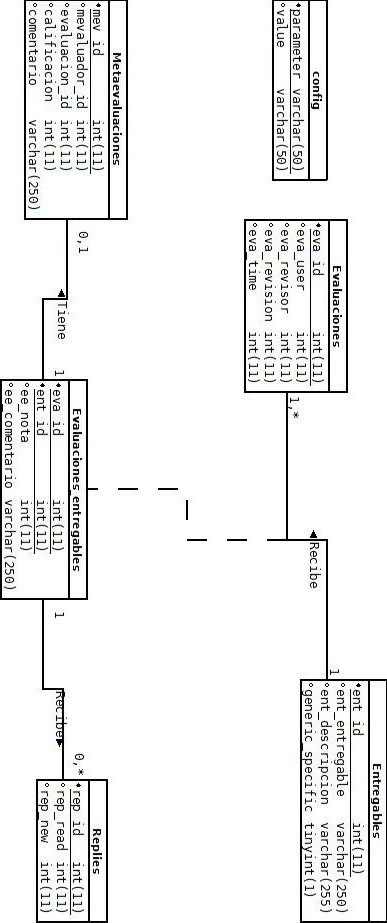
\includegraphics[width=0.6\textwidth]{db1girada.jpg}
	\caption{Diagrama de la base de datos de AMW 1.0.}
\end{figure}

\clearpage

\textbf{Base de datos 2.0}\\
	
\begin{itemize}
	\item Categorías ej ev\\
	
	En esta tabla almacenaremos información de las categorías de los ejercicios de evaluación.\\
	
	\begin{itemize}
		\item evaluation id - id del ejercicio de evaluación
		\item ent id - id de la categoría a evaluar
	\end{itemize}
	
	\item Config\\
	
	En esta tabla almacenaremos los parámetros de las configuraciones.
	
	\begin{itemize}
		\item parameter - nombre del parámetro
		\item value - valor del parámetro
	\end{itemize}
	
	\item Ejercicios de evaluación\\
	
	En esta tabla almacenaremos los distintos ejercicios de evaluación.
	
	\begin{itemize}
		\item evaluation id - id del ejercicio de evaluación
		\item exercise name - nombre del ejercicio de evaluación
		\item beginning - fecha de inicio
		\item first phase end - fin del periodo de definición de los criterios de evaluación
		\item second phase end - fin del periodo de desarrollo del ejercicio
		\item third phase end - fin del periodo de evaluación entre alumnos
		\item fourth phase end - fin de la fase final de supervisión
		\item description - descripción del ejercicio de evaluación
	\end{itemize}
	
	\item Entregables\\
	
	En esta tabla almacenaremos las categorías a evaluar en cada ejercicio.
	
	\begin{itemize}
		\item ent id - id de la categoría a evaluar
		\item ent entregale - nombre de la categoría a evaluar
		\item ent descripción - descripción de la categoría a evaluar
		\item generic specific - define si la categoría a evaluar es genérica o especifica
	\end{itemize}
	
	\item Evaluaciones\\
	
	En esta tabla almacenaremos datos de la edición una vez haya sido evaluada.
	
	\begin{itemize}
		\item eva id - id de la evaluación
		\item eva user - id del autor de la edición
		\item eva revisor - id del evaluador de la edición
		\item eva revision - id de la edición
		\item eva time - tiempo empleado en la evaluación
	\end{itemize}
	
	\item Evaluaciones entregables\\
	
	En esta tabla almacenaremos los datos de la evaluación.
	
	\begin{itemize}
		\item eva id - id de la evaluación
		\item ent id - id de la categoría evaluada
		\item ee nota - nota de la edición en una categoría
		\item ee comentario - comentarios sobre la valoración de la edición
	\end{itemize}
	
	\item Metaevaluaciones\\
	
	En esta tabla almacenaremos las metaevaluaciones realizadas.
	
	\begin{itemize}
		\item mev id - id de la metaevaluación
		\item mevaluador id - id del meta-evaluador
		\item evaluación id - id de la evaluación
		\item calificación - valoración de la evaluación
		\item comentario - comentarios sobre la valoración de la evaluación
	\end{itemize}
	
	\item Preasignaciones\\
	
	En esta tabla almacenaremos las preasignaciones realizadas.
	
	\begin{itemize}
		\item preasignación id - id de la preasignación
		\item edit id - id de la edición
		\item revisor id - id del evaluador de la edición
		\item ejercicio de evaluación - id del ejercicio de evaluación
	\end{itemize}
	
	\item Ráfagas\\
	
	En esta tabla almacenaremos las ráfagas de ediciones generadas.
	
	\begin{itemize}
		\item raf start - id de la edición donde empieza la ráfaga
		\item raf end - id de la edición donde termina la ráfaga
		\item raf timestamp - fecha y hora de la edición final
		\item raf size - tamaño de la ráfaga
	\end{itemize}
	
	\item Replies\\
	
	En esta tabla almacenaremos las re-evaluaciones solicitadas.
	
	\begin{itemize}
		\item rep id - id del reply
		\item rep read - id de la evaluación antigua
		\item rep new - id de la nueva evaluación
	\end{itemize}
	
	\item Rol assignations\\
	
	En esta tabla almacenaremos las asignaciones de roles.
	
	\begin{itemize}
		\item user id - id del usuario
		\item rol id - id del rol
	\end{itemize}
	
	\item Roles\\
	
	En esta tabla almacenaremos los roles existentes.
	
	\begin{itemize}
		\item rol id - id del rol
		\item name - nombre del rol
		\item evaluar - permisos para la sección de evaluar
		\item feedback - permisos para la sección de feedback
		\item metaevaluar - permisos para la sección de metaevaluar
		\item metaevaluar lista - permisos para la sección de la lista de metaevaluaciones
		\item alumnos - permisos para la sección de la lista de alumnos
		\item parámetros - permisos para la sección de parámetros
	\end{itemize}
	
\end{itemize}

\begin{figure}[h]
	\centering
	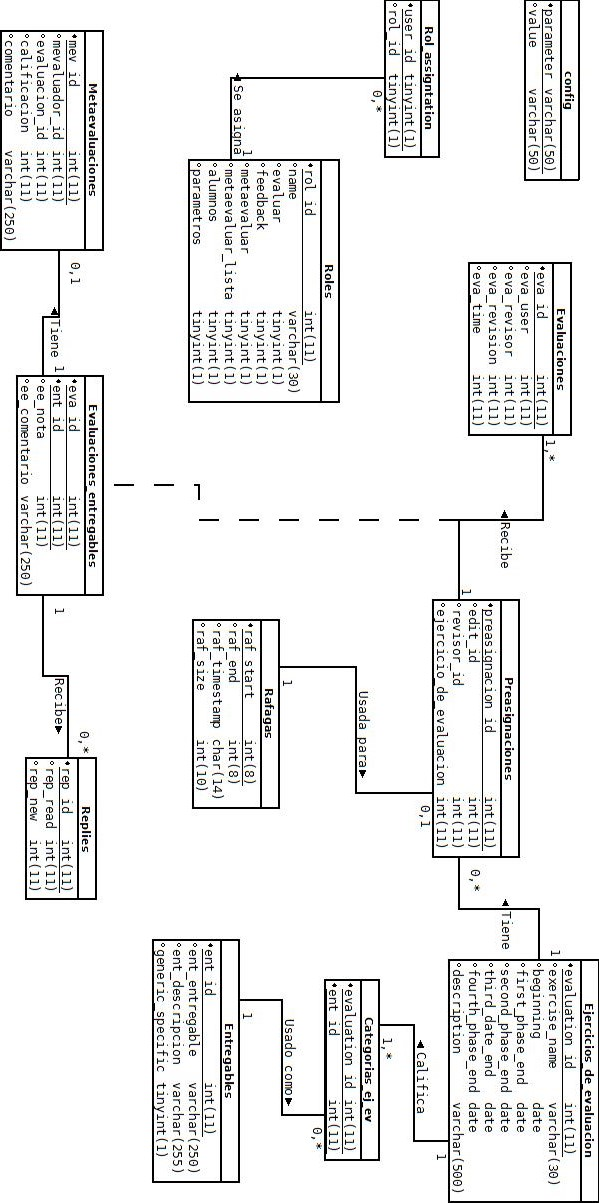
\includegraphics[width=0.6\textwidth]{db2girada.jpg}
	\caption{Diagrama de la base de datos de AMW 2.0.}
\end{figure}

\clearpage

\section{Modelo de Casos de Uso}

\begin{figure}
	\centering
	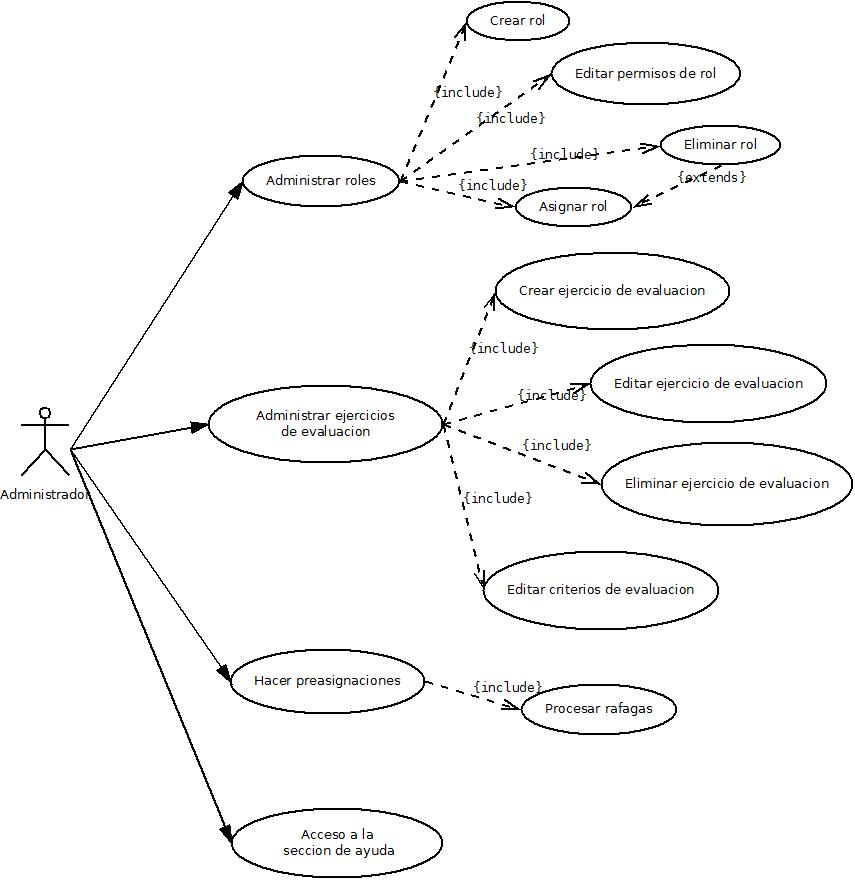
\includegraphics[width=1.0\textwidth]{Casos-de-uso.jpg}
	\caption{Modelo de casos de uso.}
\end{figure}

\subsection{Actores} 
Los actores básicos son:
\newline
- Administrador/Profesor: El usuario supervisor del sistema
\newline
- Estudiante: Usuario que realizara las evaluaciones de las ediciones suyas o de sus compañeros
\newline

Pero hay que tener en cuenta que el administrador puede crear nuevos roles, lo que generara nuevos actores dependiendo de los permisos que se les conceda a dichos roles.

\newpage

\subsection{Descripción de los casos de uso}
Caso de uso:  \textbf{Administrar roles}
\newline
Descripción: El usuario se dirige a la pagina de administración de roles.
\newline
Actores: Usuario, Sistema
\newline
Precondiciones: El usuario esta logeado y es administrador.
\newline
Postcondiciones: El sistema muestra la pagina de administración de roles.
\newline
Escenario principal:
\begin{itemize}
	\item 1. El usuario hace clic en el enlace a la administración de roles.
	\item El sistema muestra la pagina de administración de roles.
\end{itemize}

Escenario alternativo 1: 
\begin{itemize}
	\item *.* En cualquier momento del caso de uso el usuario usa los botones de navegación (atrás, adelante, actualizar) y termina el proceso actual sin guardar los datos ni ejecutarse ninguna acción.
\end{itemize}
Escenario alternativo 2:
\begin{itemize}
\item *.* En cualquier momento del caso de uso el usuario viaja a otra sección de la web o a otra web y termina el proceso actual sin guardar los datos ni ejecutarse ninguna acción.
\end{itemize}

Caso de uso: \textbf{Crear rol}
\newline
Descripción: El usuario decide crear un nuevo rol.
\newline
Actores: Usuario, Sistema
\newline
Precondiciones: El usuario esta logeado y es administrador y se encuentra en la pagina de administración de roles.
\newline
Postcondiciones: Se introduce un nuevo rol en la base de datos del sistema.
\newline
Escenario principal:
\begin{itemize}
	\item 1. El usuario rellena los datos para crear un nuevo rol en la pagina de administración de roles.
	\item 2. El usuario hace clic en crear rol.
	\item 3. El sistema comprueba que no existe ningún otro rol en el sistema con el nombre del nuevo rol a crear.
	\item 4. El sistema añade el nuevo rol a la base de datos del sistema.
 \item 5. El sistema actualiza la pagina de administración de roles, mostrando también el nuevo rol añadido.
\end{itemize}
Escenario alternativo 1: 
\begin{itemize}
	\item *.* En cualquier momento del caso de uso el usuario usa los botones de navegación (atrás, adelante, actualizar) y termina el proceso actual sin guardar los datos ni ejecutarse ninguna acción.
\end{itemize}
Escenario alternativo 2:
\begin{itemize}
	\item *.* En cualquier momento del caso de uso el usuario viaja a otra sección de la web o a otra web y termina el proceso actual sin guardar los datos ni ejecutarse ninguna acción.
\end{itemize}
Escenario alternativo 3:
\begin{itemize}
	\item 3.a El sistema detecta que el nuevo rol a introducir ya existe en el sistema.
	\item 4.a El sistema actualiza la pagina de administración de roles, sin añadir el nuevo rol que el usuario pretendía añadir.
\end{itemize}

Caso de uso: \textbf{Editar permisos de rol}
\newline
Descripción: El usuario decide editar los permisos de un rol.
\newline
Actores: Usuario, Sistema
\newline
Precondiciones: El usuario esta logeado y es administrador y se encuentra en la pagina de administración de roles.
\newline
Postcondiciones: Se modifican los permisos de un rol en la base de datos del sistema.
\newline
Escenario principal:
\begin{itemize}
\item 1. El usuario rellena los datos para modificar los permisos de un rol en la pagina de administración de roles.
\item 2. El usuario hace clic en modificar rol.
\item 3. El sistema modifica los permisos del rol en la base de datos del sistema.
\item 4. El sistema actualiza la pagina de administración de roles, mostrando los cambios efectuados.
\end{itemize}
Escenario alternativo 1: 
\begin{itemize}
	\item *.* En cualquier momento del caso de uso el usuario usa los botones de navegación (atrás, adelante, actualizar) y termina el proceso actual sin guardar los datos ni ejecutarse ninguna acción.
\end{itemize}
Escenario alternativo 2:
\begin{itemize}
	\item *.* En cualquier momento del caso de uso el usuario viaja a otra sección de la web o a otra web y termina el proceso actual sin guardar los datos ni ejecutarse ninguna acción.
\end{itemize}

Caso de uso: \textbf{Eliminar rol}
\newline
Descripción: El usuario decide eliminar rol.
\newline
Actores: Usuario, Sistema
\newline
Precondiciones: El usuario esta logeado y es administrador y se encuentra en la pagina de administración de roles.
\newline
Postcondiciones: Se elimina el rol seleccionado de la base de datos del sistema.
\newline
Escenario principal:
\begin{itemize}
	\item 1. El sistema muestra una lista desplegable con los roles existentes en el sistema, exceptuando los de administrador y estudiante.
	\item 2. El usuario selecciona el rol que desea eliminar.
	\item 3. El usuario hace clic en el botón de eliminar rol.
	\item 4. El sistema elimina todas las asignaciones de usuarios al rol a eliminar.
	\item 5. El sistema elimina el rol seleccionado de la base de datos del sistema.
	\item 6. El sistema actualiza la pagina de administración de roles, mostrando los cambios efectuados.
\end{itemize}
Escenario alternativo 1:
\begin{itemize} 
	\item *.* En cualquier momento del caso de uso el usuario usa los botones de navegación (atrás, adelante, actualizar) y termina el proceso actual sin guardar los datos ni ejecutarse ninguna acción.
\end{itemize}
Escenario alternativo 2:
\begin{itemize}
	\item *.* En cualquier momento del caso de uso el usuario viaja a otra sección de la web o a otra web y termina el proceso actual sin guardar los datos ni ejecutarse ninguna acción.
\end{itemize}

Caso de uso: \textbf{Asignar rol}
\newline
Descripción: El usuario decide asignar un rol a un estudiante.
\newline
Actores: Usuario, Sistema
\newline
Precondiciones: El usuario esta logeado y es administrador y se encuentra en la pagina de administración de roles.
\newline
Postcondiciones: Se introduce un nuevo rol en la base de datos del sistema.
\newline
Escenario principal:
\begin{itemize}
	\item 1. El sistema muestra una lista desplegable con los usuarios existentes en el sistema y otra con los roles existentes en el sistema.
	\item 2. El usuario selecciona un usuario y un rol de las listas.
	\item 3. El usuario hace clic en el botón de asignar rol.
	\item 4. El sistema comprueba que el usuario no tenia ningún rol asignado.
	\item 5. El sistema introduce los datos del usuario seleccionado y el rol que se le va a asignar.
	\item 6. El sistema actualiza la pagina de administración de roles, mostrando los cambios efectuados.
\end{itemize}
Escenario alternativo 1: 
\begin{itemize}
	\item *.* En cualquier momento del caso de uso el usuario usa los botones de navegación (atrás, adelante, actualizar) y termina el proceso actual sin guardar los datos ni ejecutarse ninguna acción.
\end{itemize}
Escenario alternativo 2:
\begin{itemize}
	\item *.* En cualquier momento del caso de uso el usuario viaja a otra sección de la web o a otra web y termina el proceso actual sin guardar los datos ni ejecutarse ninguna acción.
\end{itemize}
Escenario alternativo 3:
\begin{itemize}
	\item 4.a El sistema detecta que el usuario ya tiene un rol asignado.
	\item 5.a El sistema detecta que el nuevo rol que se le quiere asignar es el de estudiante.
	\item 7.a El sistema borra de la base de datos la asignación previa que tuviera el usuario seleccionado.
	\item 8.a El sistema actualiza la pagina de administración de roles, mostrando los cambios efectuados.
\end{itemize}
Escenario alternativo 4:
\begin{itemize}
	\item 5.b El sistema detecta que el nuevo rol que se quiere asignar no es el de estudiante.
	\item 6.b El sistema actualiza la base de datos con los nuevos datos introducidos
	\item 7.b El sistema actualiza la pagina de administración de roles mostrando los cambios efectuados.
\end{itemize}

Caso de uso: \textbf{Administrar ejercicios de evaluación}
\newline
Descripción: El usuario se dirige a la pagina de administración de ejercicios de evaluación
\newline
Actores: Usuario, Sistema
\newline
Precondiciones: El usuario esta logeado y es administrador.
\newline
Postcondiciones: El sistema muestra la pagina de administración de ejercicios de evaluación
\newline
Escenario principal:
\begin{itemize}
	\item 1. El usuario hace clic en el enlace a la administración de ejercicios de evaluación
	\item 2. El sistema muestra la pagina de administración de ejercicios de evaluación
\end{itemize}
Escenario alternativo 1: 
\begin{itemize}
	\item *.* En cualquier momento del caso de uso el usuario usa los botones de navegación (atrás, adelante, actualizar) y termina el proceso actual sin guardar los datos ni ejecutarse ninguna acción.
\end{itemize}
Escenario alternativo 2: 
\begin{itemize}
	\item *.* En cualquier momento del caso de uso el usuario viaja a otra sección de la web o a otra web y termina el proceso actual sin guardar los datos ni ejecutarse ninguna acción.
\end{itemize}

Caso de uso: \textbf{Crear ejercicio de evaluación}
\newline
Descripción: El usuario decide crear un nuevo ejercicio de evaluación
\newline
Actores: Usuario, Sistema
\newline
Precondiciones: El usuario esta logeado y es administrador y se encuentra en la pagina de administración de ejercicios de evaluación
\newline
Postcondiciones: Se introduce un nuevo ejercicio de evaluación en la base de datos del sistema.
\newline
Escenario principal:
\begin{itemize}
	\item 1. El usuario rellena los datos para crear un nuevo ejercicio de evaluación en la pagina de administración de ejercicios de evaluación
	\item 2. El usuario hace clic en crear ejercicio de evaluación
	\item 3. El sistema comprueba que no existe ningún otro ejercicio de evaluación en el sistema con el nombre del nuevo ejercicio de evaluación a crear.
	\item 4. El sistema añade el nuevo ejercicio de evaluación a la base de datos del sistema.
	\item 5. El sistema actualiza la pagina de administración de ejercicios de evaluación, mostrando también el nuevo ejercicio de evaluación añadido.
\end{itemize}
Escenario alternativo 1: 
\begin{itemize}
	\item *.* En cualquier momento del caso de uso el usuario usa los botones de navegación (atrás, adelante, actualizar) y termina el proceso actual sin guardar los datos ni ejecutarse ninguna acción.
\end{itemize}
Escenario alternativo 2:
\begin{itemize}
	\item *.* En cualquier momento del caso de uso el usuario viaja a otra sección de la web o a otra web y termina el proceso actual sin guardar los datos ni ejecutarse ninguna acción.
\end{itemize}
Escenario alternativo 3:
\begin{itemize}
	\item 3.a El sistema detecta que el nuevo ejercicio de evaluación a introducir ya existe en el sistema.
	\item 4.a El sistema actualiza la pagina de administración de ejercicios de evaluación, sin añadir el nuevo ejercicio de evaluación que el usuario pretendía añadir.
\end{itemize}

Caso de uso: \textbf{Editar ejercicio de evaluación}
\newline
Descripción: El usuario decide editar un ejercicio de evaluación
\newline
Actores: Usuario, Sistema
\newline
Precondiciones: El usuario esta logeado y es administrador y se encuentra en la pagina de administración de ejercicios de evaluación
\newline
Postcondiciones: Se modifican un ejercicio de evaluación en la base de datos del sistema.
\newline
Escenario principal:
\begin{itemize}
	\item 1. El usuario rellena los datos para modificar un ejercicio de evaluación en la pagina de administración de roles.
	\item 2. El usuario hace clic en modificar ejercicio de evaluación
	\item 4. El sistema modifica el ejercicio de evaluación en la base de datos del sistema.
	\item 5. El sistema actualiza la pagina de administración de ejercicios de evaluación, mostrando los cambios efectuados.
\end{itemize}
Escenario alternativo 1: 
\begin{itemize}
	\item *.* En cualquier momento del caso de uso el usuario usa los botones de navegación (atrás, adelante, actualizar) y termina el proceso actual sin guardar los datos ni ejecutarse ninguna acción.
\end{itemize}
Escenario alternativo 2:
\begin{itemize}
	\item *.* En cualquier momento del caso de uso el usuario viaja a otra sección de la web o a otra web y termina el proceso actual sin guardar los datos ni ejecutarse ninguna acción.
\end{itemize}

Caso de uso: \textbf{Eliminar ejercicio de evaluación}
\newline
Descripción: El usuario decide eliminar un ejercicio de evaluación
\newline
Actores: Usuario, Sistema
\newline
Precondiciones: El usuario esta logeado y es administrador y se encuentra en la pagina de administración de ejercicio de evaluación
\newline
Postcondiciones: Se elimina el ejercicio de evaluación seleccionado de la base de datos del sistema.
\newline
Escenario principal:
\begin{itemize}
	\item 1. El sistema muestra una lista desplegable con los ejercicios de evaluación existentes en el sistema.
	\item 2. El usuario selecciona el ejercicio de evaluación que desea eliminar.
	\item 3. El usuario hace clic en el botón de eliminar ejercicio de evaluación
	\item 4. El sistema elimina el ejercicio de evaluación seleccionado de la base de datos del sistema.
	\item 5. El sistema actualiza la pagina de administración de ejercicios de evaluación, mostrando los cambios efectuados.
\end{itemize}
Escenario alternativo 1: 
\begin{itemize}
	\item *.* En cualquier momento del caso de uso el usuario usa los botones de navegación (atrás, adelante, actualizar) y termina el proceso actual sin guardar los datos ni ejecutarse ninguna acción.
\end{itemize}
Escenario alternativo 2:
\begin{itemize}
	\item *.* En cualquier momento del caso de uso el usuario viaja a otra sección de la web o a otra web y termina el proceso actual sin guardar los datos ni ejecutarse ninguna acción.
\end{itemize}

Caso de uso: \textbf{Editar criterios de evaluación}
\newline
Descripción: El usuario decide editar los criterios de evaluación de un ejercicio de evaluación
\newline
Actores: Usuario, Sistema
\newline
Precondiciones: El usuario esta logeado y es administrador y se encuentra en la pagina de administración de ejercicio de evaluación
\newline
Postcondiciones: Se modifican los criterios de evaluación de un ejercicio de evaluación en la base de datos del sistema.
\newline
Escenario principal:
\begin{itemize}
	\item 1. El sistema muestra una tabla con los ejercicio de evaluación y criterios de evaluación existentes en el sistema.
	\item 2. El usuario modifica los criterios de evaluación de uno de los ejercicios de evaluación
	\item 3. El usuario hace clic en el botón de modificar criterios de evaluación
	\item 4. El sistema modifica los datos para el ejercicio de evaluación seleccionado.
	\item 5. El sistema actualiza la pagina de administración de roles, mostrando los cambios efectuados.
\end{itemize}
Escenario alternativo 1: 
\begin{itemize}
	\item *.* En cualquier momento del caso de uso el usuario usa los botones de navegación (atrás, adelante, actualizar) y termina el proceso actual sin guardar los datos ni ejecutarse ninguna acción.
\end{itemize}
Escenario alternativo 2:
\begin{itemize}
	\item *.* En cualquier momento del caso de uso el usuario viaja a otra sección de la web o a otra web y termina el proceso actual sin guardar los datos ni ejecutarse ninguna acción.
\end{itemize}

Caso de uso: \textbf{Hacer Preasignaciones}
\newline
Descripción: El usuario decide realizar las preasignaciones para un ejercicio de evaluación
\newline
Actores: Usuario, Sistema
\newline
Precondiciones: El usuario esta logeado y es administrador y se encuentra en la pagina de administración de ejercicio de evaluación
\newline
Postcondiciones: Se realizan las preasignaciones para un ejercicio de evaluación
\newline
Escenario principal:
\begin{itemize}
	\item 1. El sistema muestra una lista desplegable con los ejercicio de evaluación para los cuales aun no se han realizado preasignaciones existentes en el sistema.
	\item 2. El usuario selecciona uno de los ejercicios de evaluación
	\item 3. El usuario hace clic en el botón de hacer preasignaciones
	\item 4. El sistema realiza el procesado de ráfagas y posteriormente asigna las ediciones del ejercicio de evaluación a los Estudiantes según la configuración del sistema.
	\item 5. El sistema actualiza la pagina de administración de ejercicios de evaluación, mostrando los cambios efectuados.
\end{itemize}
Escenario alternativo 1: 
\begin{itemize}
	\item *.* En cualquier momento del caso de uso el usuario usa los botones de navegación (atrás, adelante, actualizar) y termina el proceso actual sin guardar los datos ni ejecutarse ninguna acción.
\end{itemize}
Escenario alternativo 2:
\begin{itemize}
	\item *.* En cualquier momento del caso de uso el usuario viaja a otra sección de la web o a otra web y termina el proceso actual sin guardar los datos ni ejecutarse ninguna acción.
\end{itemize}

Caso de uso: \textbf{Procesar ráfagas}
\newline
Descripción: Se procesan las posibles ráfagas existentes en el sistema
\newline
Actores: Sistema
\newline
Precondiciones: El usuario selecciona la opción de hacer preasignaciones.
\newline
Postcondiciones: Se analizan las ediciones existentes y se crean las ráfagas que procedan.
\newline
Escenario principal:
\begin{itemize}
	\item 1. El sistema busca en cada pagina todas las ediciones realizadas en el plazo establecido.
	\item 2. El sistema detecta que 2 ediciones consecutivas han sido realizadas en menos de el periodo de tiempo establecido por el mismo usuario.
	\item 3. El sistema crea una ráfaga o añade la ultima edición a una ráfaga existente.
\end{itemize}

\newpage

\section{Modelo de Comportamiento}

En las siguientes imágenes podemos ver los modelos de comportamiento:
\newline

\begin{figure}[h!]
	\centering
	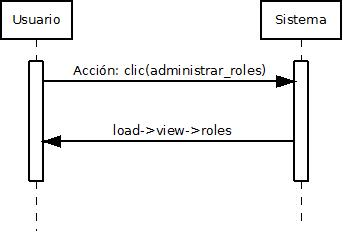
\includegraphics[width=0.6\textwidth]{ds_administrar_roles.jpg}
	\caption{Caso de uso: administrar roles.}
\end{figure}

\begin{figure}
	\centering
	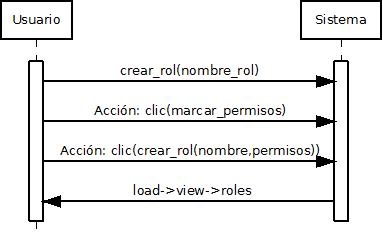
\includegraphics[width=0.6\textwidth]{ds_crear_rol.jpg}
	\caption{Caso de uso: crear rol.}
\end{figure}

\begin{figure}
	\centering
	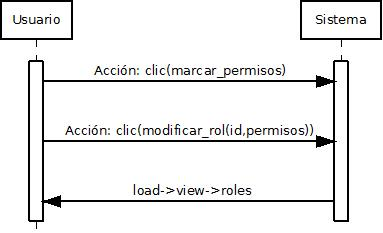
\includegraphics[width=0.6\textwidth]{ds_modificar_rol.jpg}
	\caption{Caso de uso: editar permisos de rol.}
\end{figure}

\begin{figure}
	\centering
	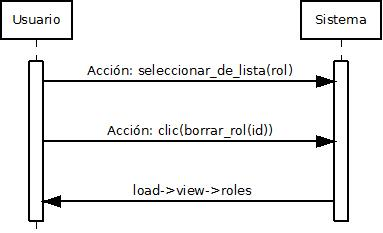
\includegraphics[width=0.6\textwidth]{ds_eliminar_rol.jpg}
	\caption{Caso de uso: eliminar rol.}
\end{figure}

\begin{figure}
	\centering
	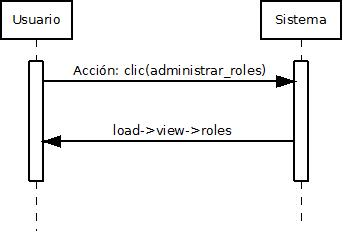
\includegraphics[width=0.6\textwidth]{ds_administrar_roles.jpg}
	\caption{Caso de uso: asignar rol.}
\end{figure}

\begin{figure}
	\centering
	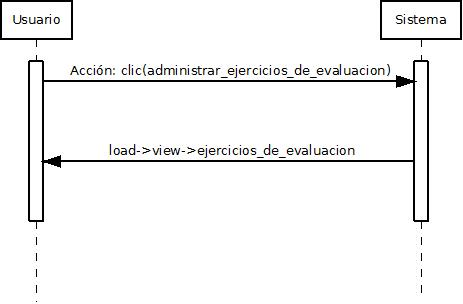
\includegraphics[width=0.6\textwidth]{ds_administrar_ejercicios_evaluacion.jpg}
	\caption{Caso de uso: administrar ejercicios de evaluación.}
\end{figure}

\begin{figure}
	\centering
	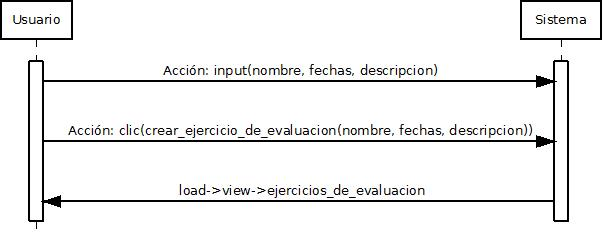
\includegraphics[width=0.6\textwidth]{ds_crear_ejercicio_evaluacion.jpg}
	\caption{Caso de uso: crear ejercicio de evaluación.}
\end{figure}

\begin{figure}
	\centering
	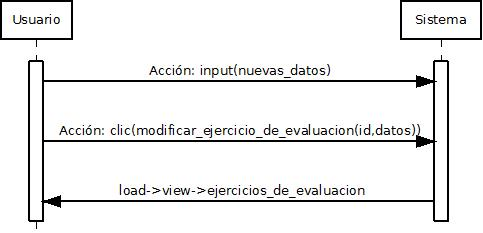
\includegraphics[width=0.6\textwidth]{ds_modificar_ejercicio_evaluacion.jpg}
	\caption{Caso de uso: editar ejercicio de evaluación.}
\end{figure}

\begin{figure}
	\centering
	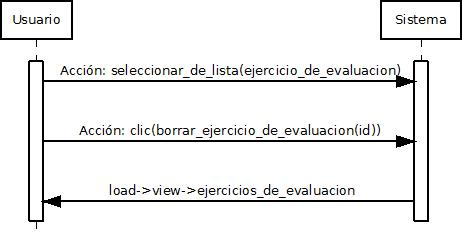
\includegraphics[width=0.6\textwidth]{ds_eliminar_ejercicio_evaluacion.jpg}
	\caption{Caso de uso: eliminar ejercicio de evaluación.}
\end{figure}

\begin{figure}
	\centering
	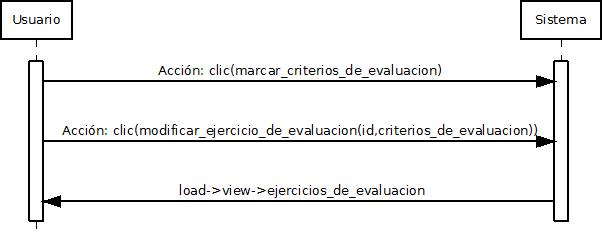
\includegraphics[width=0.6\textwidth]{ds_editar_criterios_de_evaluacion.jpg}
	\caption{Caso de uso: editar criterios de evaluación.}
\end{figure}

\begin{figure}
	\centering
	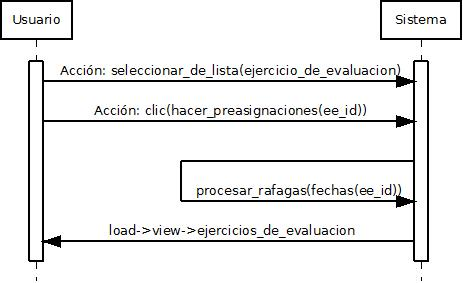
\includegraphics[width=0.6\textwidth]{ds_hacer_preasignaciones.jpg}
	\caption{Caso de uso: hacer preasignaciones.}
\end{figure}

\begin{figure}
	\centering
	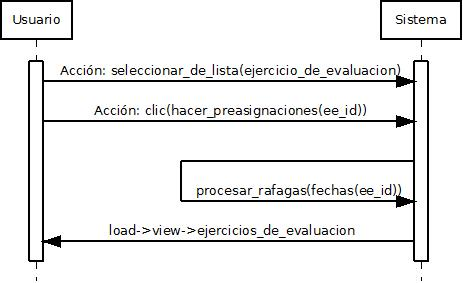
\includegraphics[width=0.6\textwidth]{ds_procesar_rafagas.jpg}
	\caption{Caso de uso: procesar ráfagas.}
\end{figure}

\begin{figure}
	\centering
	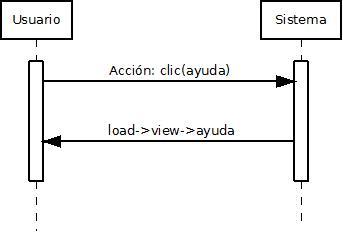
\includegraphics[width=0.6\textwidth]{ds_acceso_ayuda.jpg}
	\caption{Caso de uso: acceso a ayuda.}
\end{figure}

\newpage

\section{Modelo de Interfaz de Usuario}

En esta sección se detalla la navegación entre pantallas adjuntando imágenes de la interfaz del sistema, la principal forma de navegación es a través del menú superior.\\

A continuación se muestra la pantalla de inicio de sesión, en la cual es usuario debe introducir sus datos para acceder al sistema.\\

\begin{figure}[h!]
	\centering
	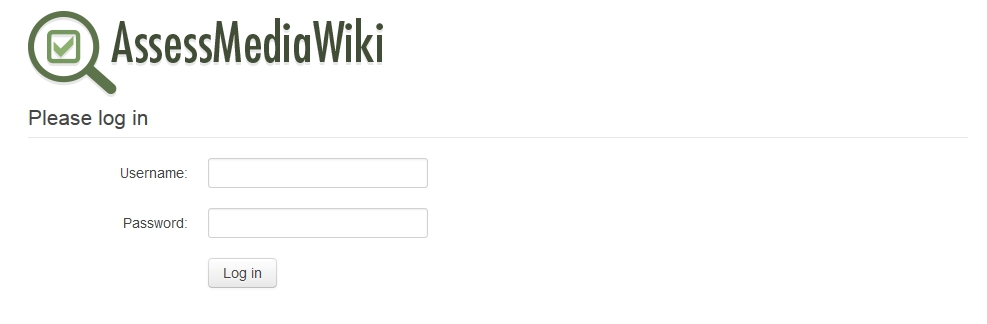
\includegraphics[width=0.9\textwidth]{sc_login.jpg}
	\caption{Pantalla de login.}
\end{figure}
\clearpage

Una vez iniciada sesión aparece la pantalla de inicio, donde aparecerán las evaluaciones disponibles para el usuario en casi de que hubiese, en cualquier momento podemos volver a esta pantalla haciendo clic en el botón "Assess" del menú superior.\\

\begin{figure}[h!]
	\centering
	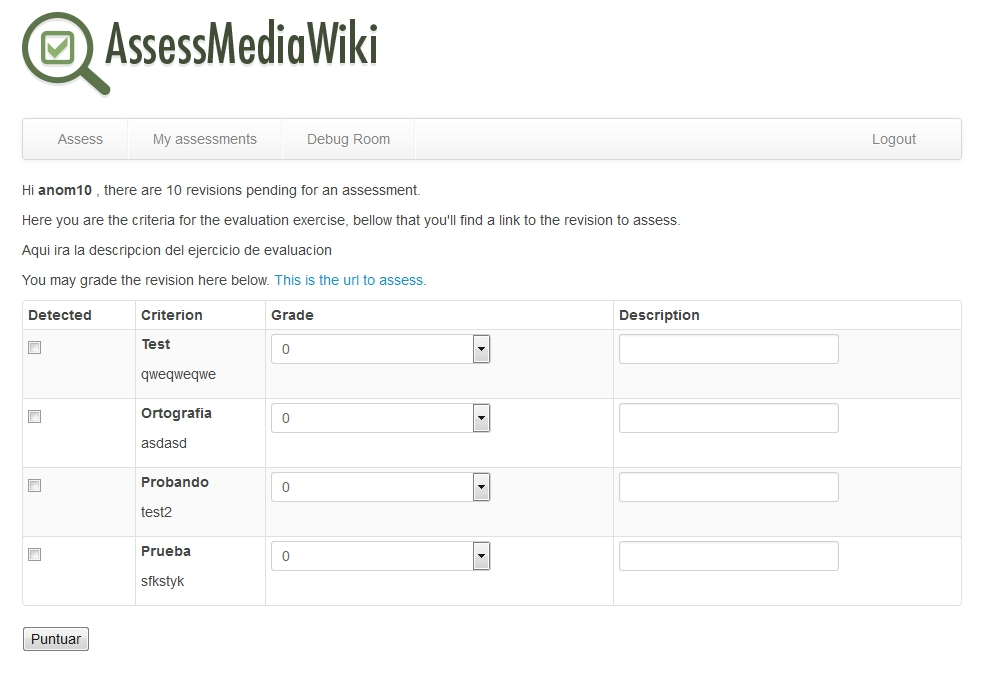
\includegraphics[width=0.9\textwidth]{sc_revision.jpg}
	\caption{Pantalla de inicio del usuario (sin la sala de debug, eso es debido a que el modo de desarrollo esta activado).}
\end{figure}
\clearpage

En caso de no haber evaluaciones disponibles para el usuario aparecerá el siguiente mensaje en la pagina principal.\\

\begin{figure}[h!]
	\centering
	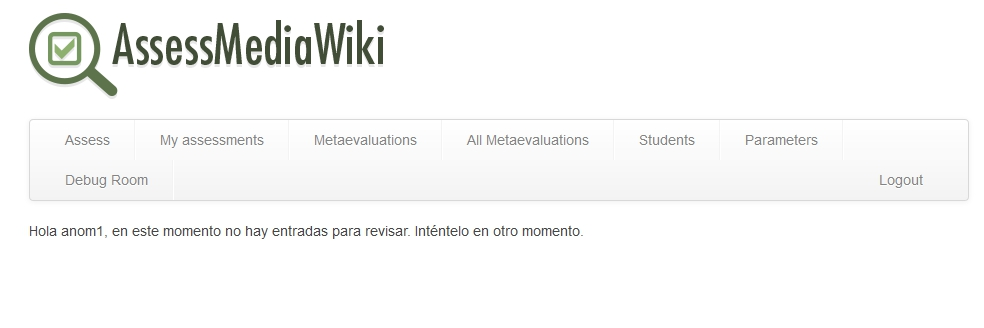
\includegraphics[width=0.9\textwidth]{sc_no_revision.jpg}
	\caption{Pantalla de usuario sin revisiones.}
\end{figure}
\clearpage

A partir de este punto usaremos capturas de pantalla con el perfil de profesor / administrador, ya que es el rol que tiene permisos para acceder a todas las secciones del sistema, los estudiantes tendrían los permisos básicos mostrados previamente.\\

A continuación se muestra la pantalla de metaevaluaciones, que estará disponible a trabes del botón "Metaevaluations" en el menú superior, para el profesor / administrador y para todos aquellos roles que el profesor / administrador lo haya habilitado.\\

\begin{figure}[h!]
	\centering
	\includegraphics[width=0.9\textwidth]{sc_metaevaluar.jpg}
	\caption{Pantalla de metaevaluaciones.}
\end{figure}
\clearpage

Si hacemos clic en el apartado del menú "All metaevaluations" podremos ver la lista completa de todas las metaevaluaciones realizadas existentes en el sistema, como podemos ver a continuacion.\\

\begin{figure}[h!]
	\centering
	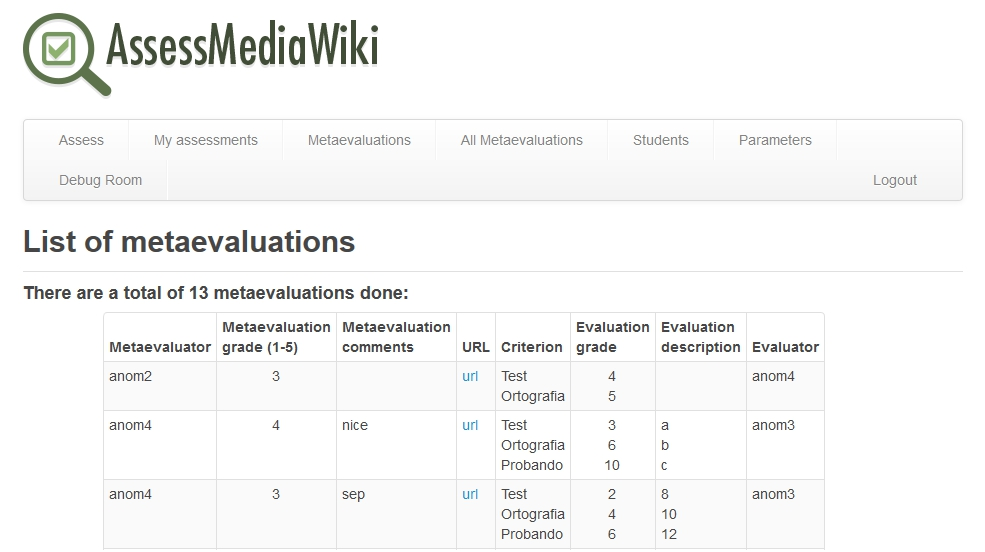
\includegraphics[width=0.9\textwidth]{sc_metaevaluar_lista.jpg}
	\caption{Pantalla de listado de metaevaluaciones.}
\end{figure}
\clearpage

Si hacemos clic en el apartado del menú "Students" podremos ver la lista completa de todos los estudiantes existentes en el sistema, y a través de los enlaces "Report", "Metaevaluations resume" y "CSV" podremos ver información detallada sobre las evaluaciones de los alumnos, las metaevaluaciones realizadas y generas un CSV (Coma Separated Values) respectivamente.\\

\begin{figure}[h!]
	\centering
	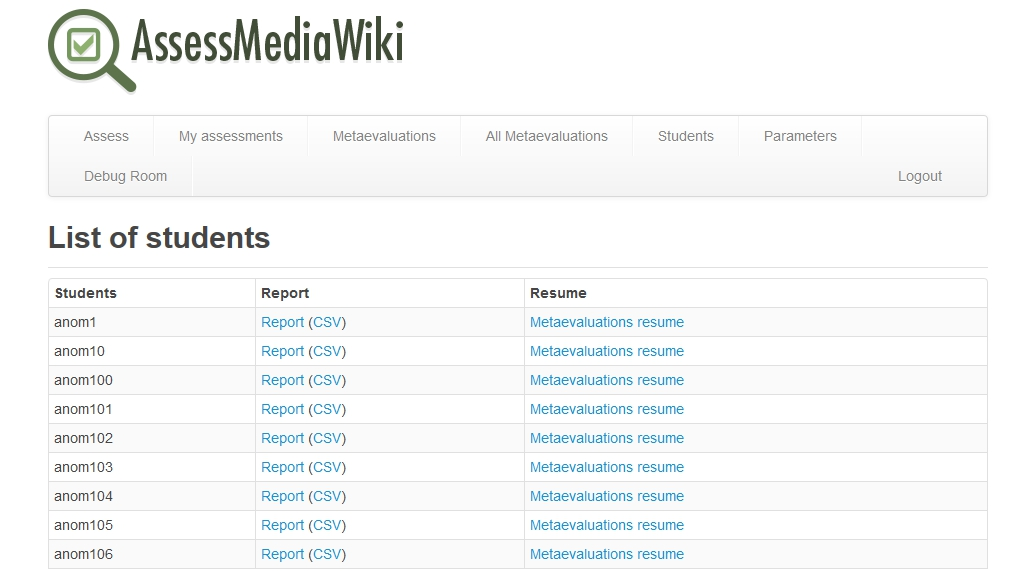
\includegraphics[width=0.9\textwidth]{sc_student_list.jpg}
	\caption{Pantalla de listado de alumnos.}
\end{figure}
\clearpage

Al hacer clic en el botón "Parameters" en el menú superior podremos acceder a configuraciones del sistema como vemos a continuacion.\\

Al final de la lista de parámetros encontraremos los botones "Administration of evaluation exercises", "Administration of roles" y "Help", funciones añadidas en esta nueva versión de AssessMediaWiki, cuyas interfaces veremos a continuacion.

\begin{figure}[h!]
	\centering
	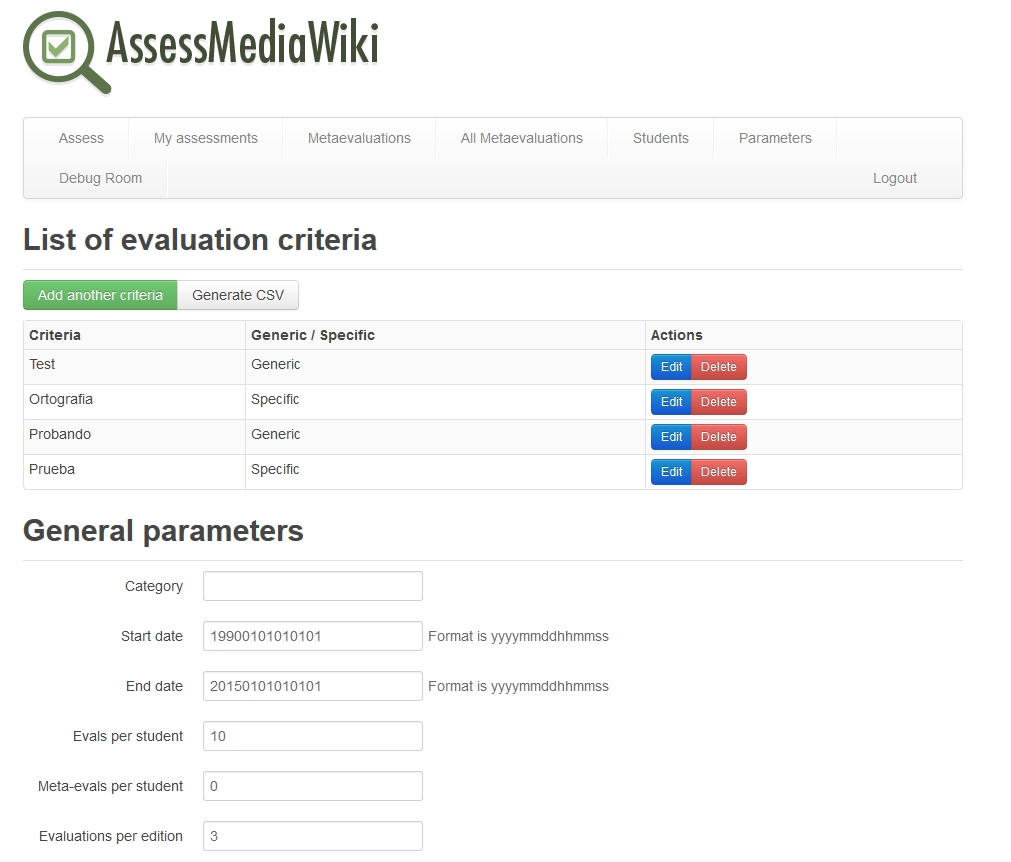
\includegraphics[width=0.9\textwidth]{sc_parametros1.jpg}
	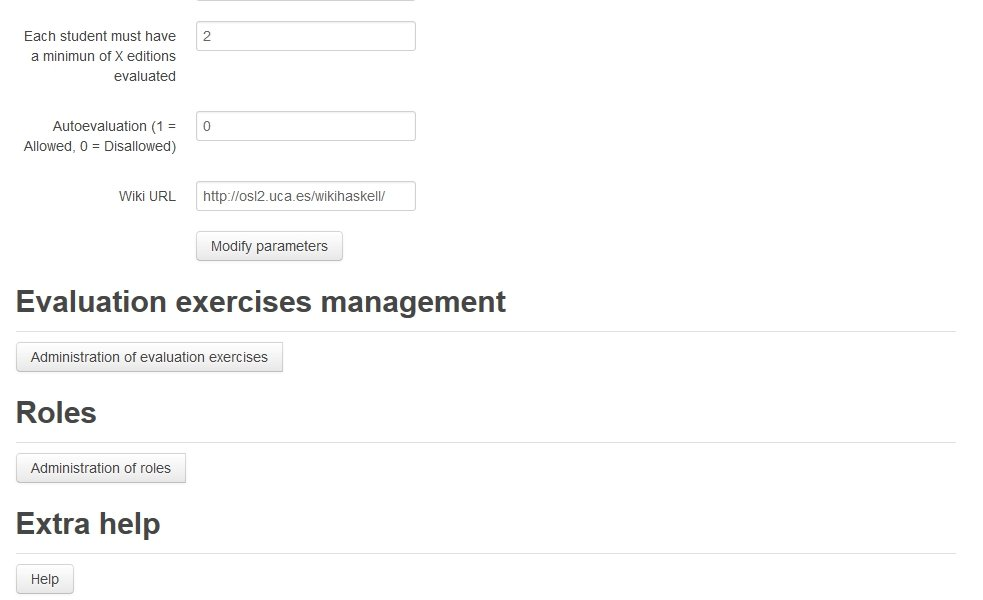
\includegraphics[width=0.9\textwidth]{sc_parametros2.jpg}
	\caption{Pantalla de parámetros.}
\end{figure}
\clearpage

A continuación veremos la interfaz de administración de roles, accesible desde el botón "Administration of roles" al final del listado de parámetros, a través de esta interfaz podremos crear nuevos roles, eliminar roles obsoletos, administrar los permisos de los roles existentes, asignar roles a los usuarios y ver que usuarios tienen roles asignados.\\

\begin{figure}[h!]
	\centering
	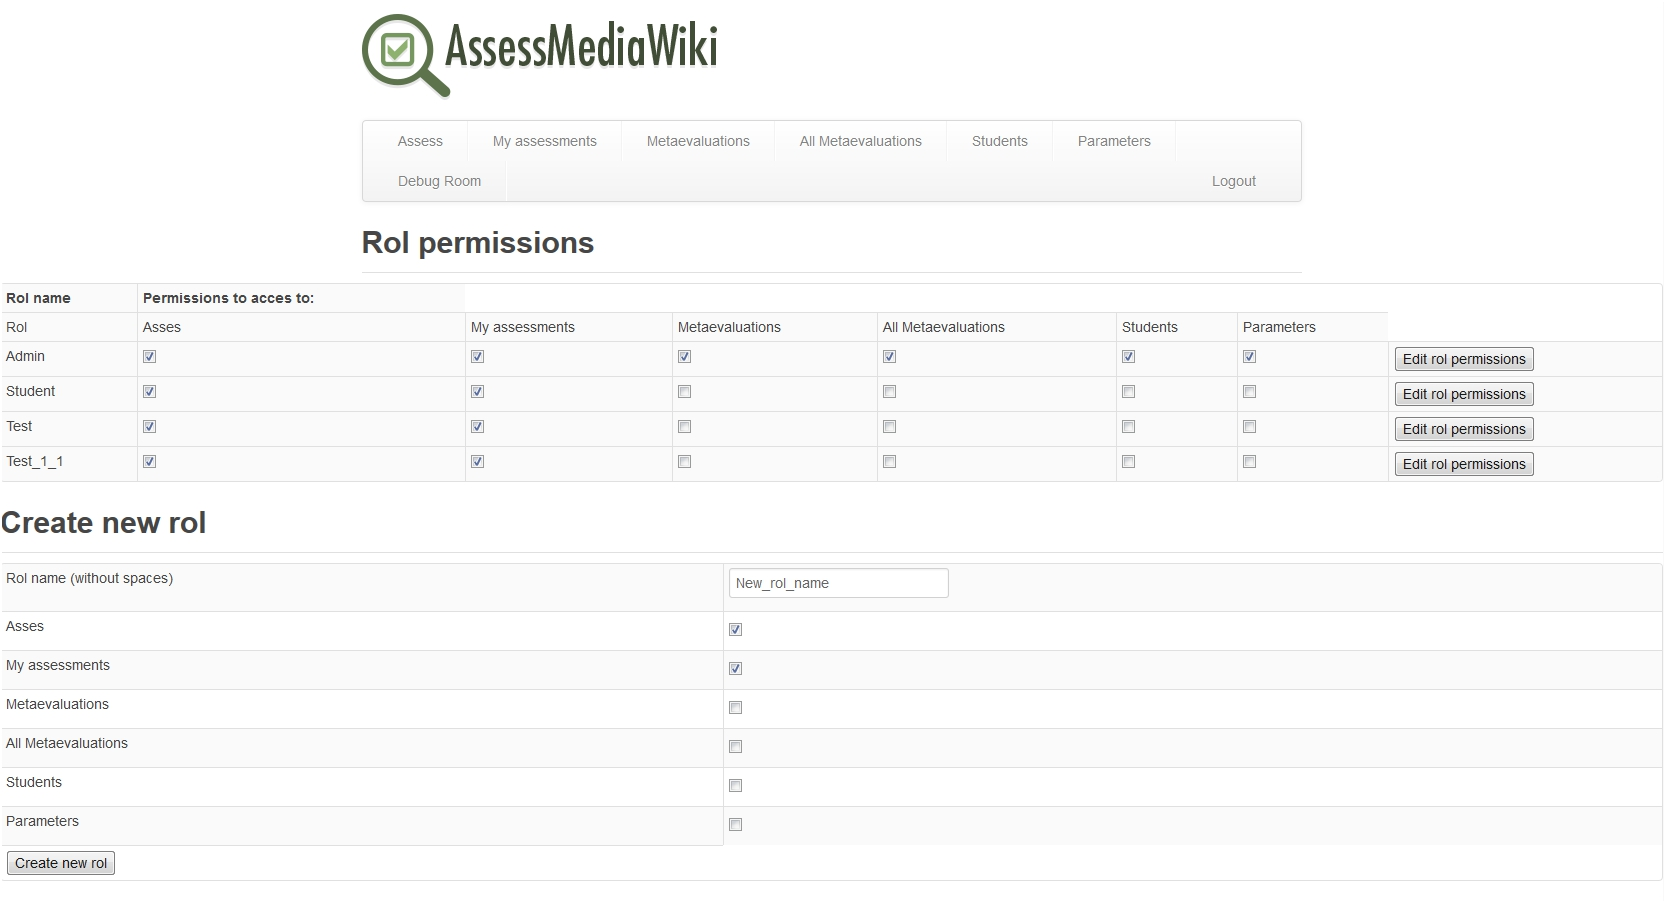
\includegraphics[width=0.9\textwidth]{sc_roles1.jpg}
	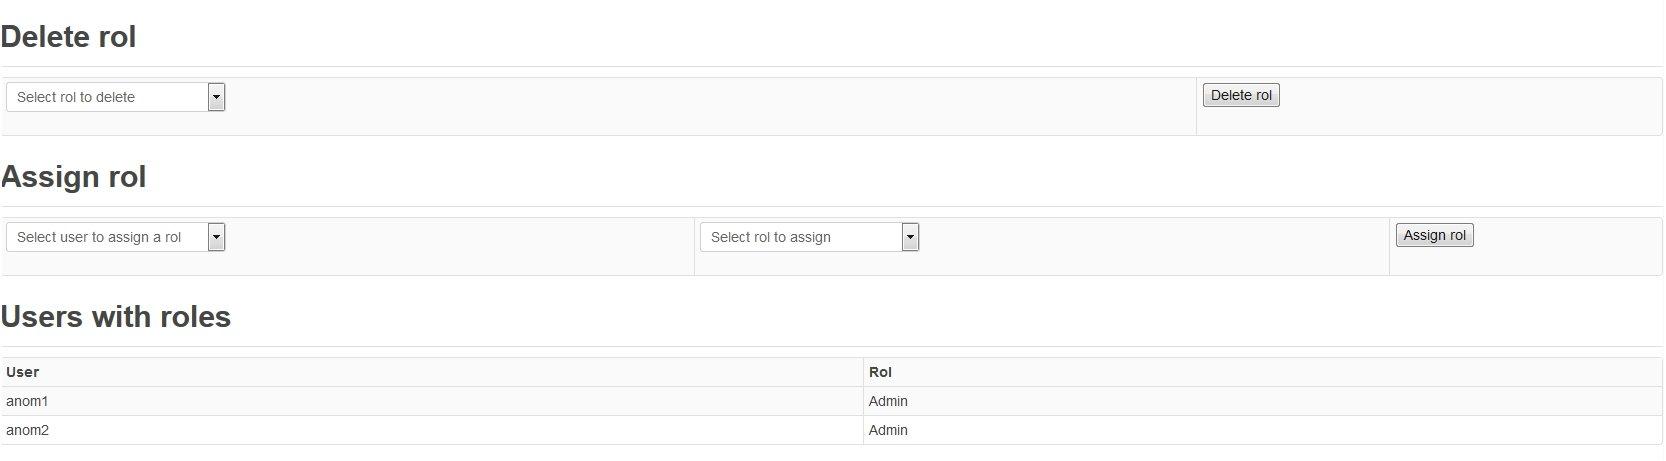
\includegraphics[width=0.9\textwidth]{sc_roles2.jpg}
	\caption{Pantalla de configuración de roles.}
\end{figure}
\clearpage

A continuación veremos la interfaz de administración de ejercicios de evaluación, accesible desde el botón "Administration of evaluation exercises" al final del listado de parámetros, a través de esta interfaz podremos crear nuevos ejercicios de evaluación, eliminar ejercicios de evaluación, administrar los parámetros de los ejercicios de evaluación existentes, modificar las categorías a evaluar en los ejercicios de evaluación correspondientes.\\

\begin{figure}[h!]
	\centering
	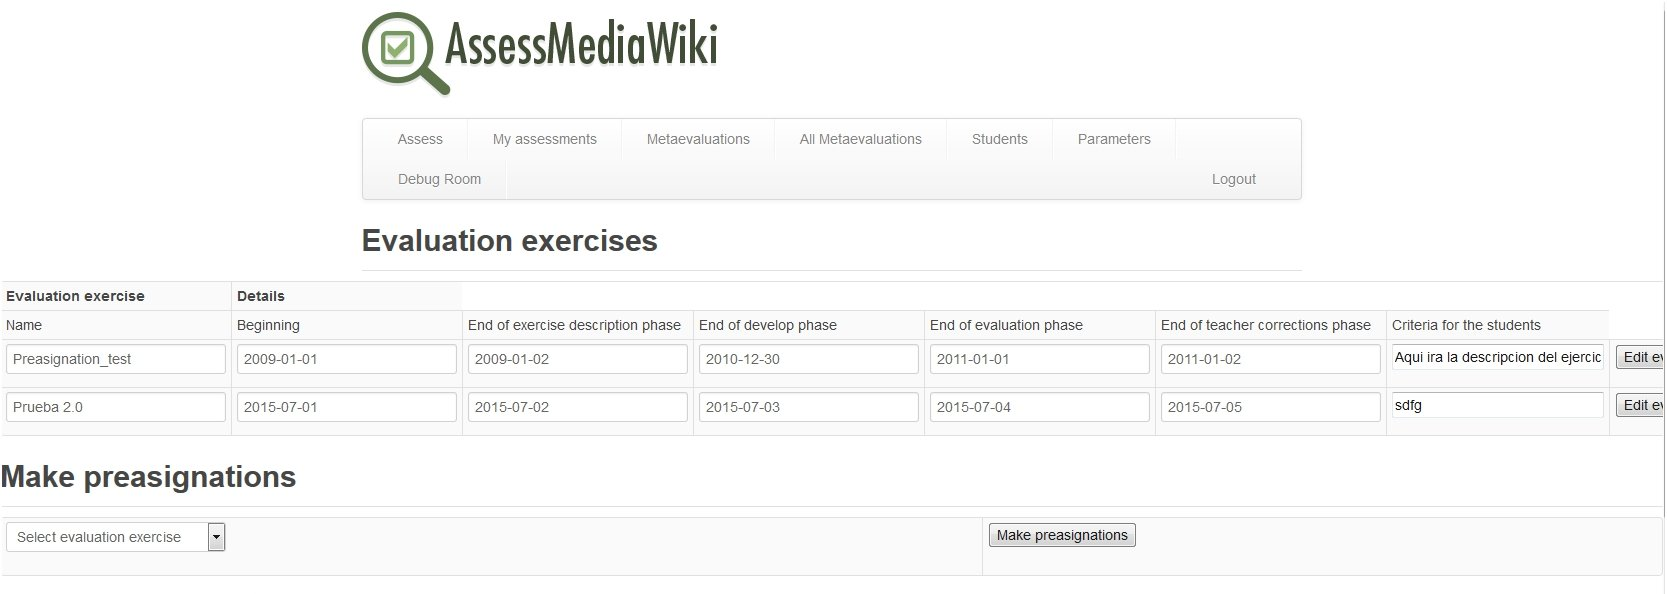
\includegraphics[width=0.9\textwidth]{sc_ee1.jpg}
	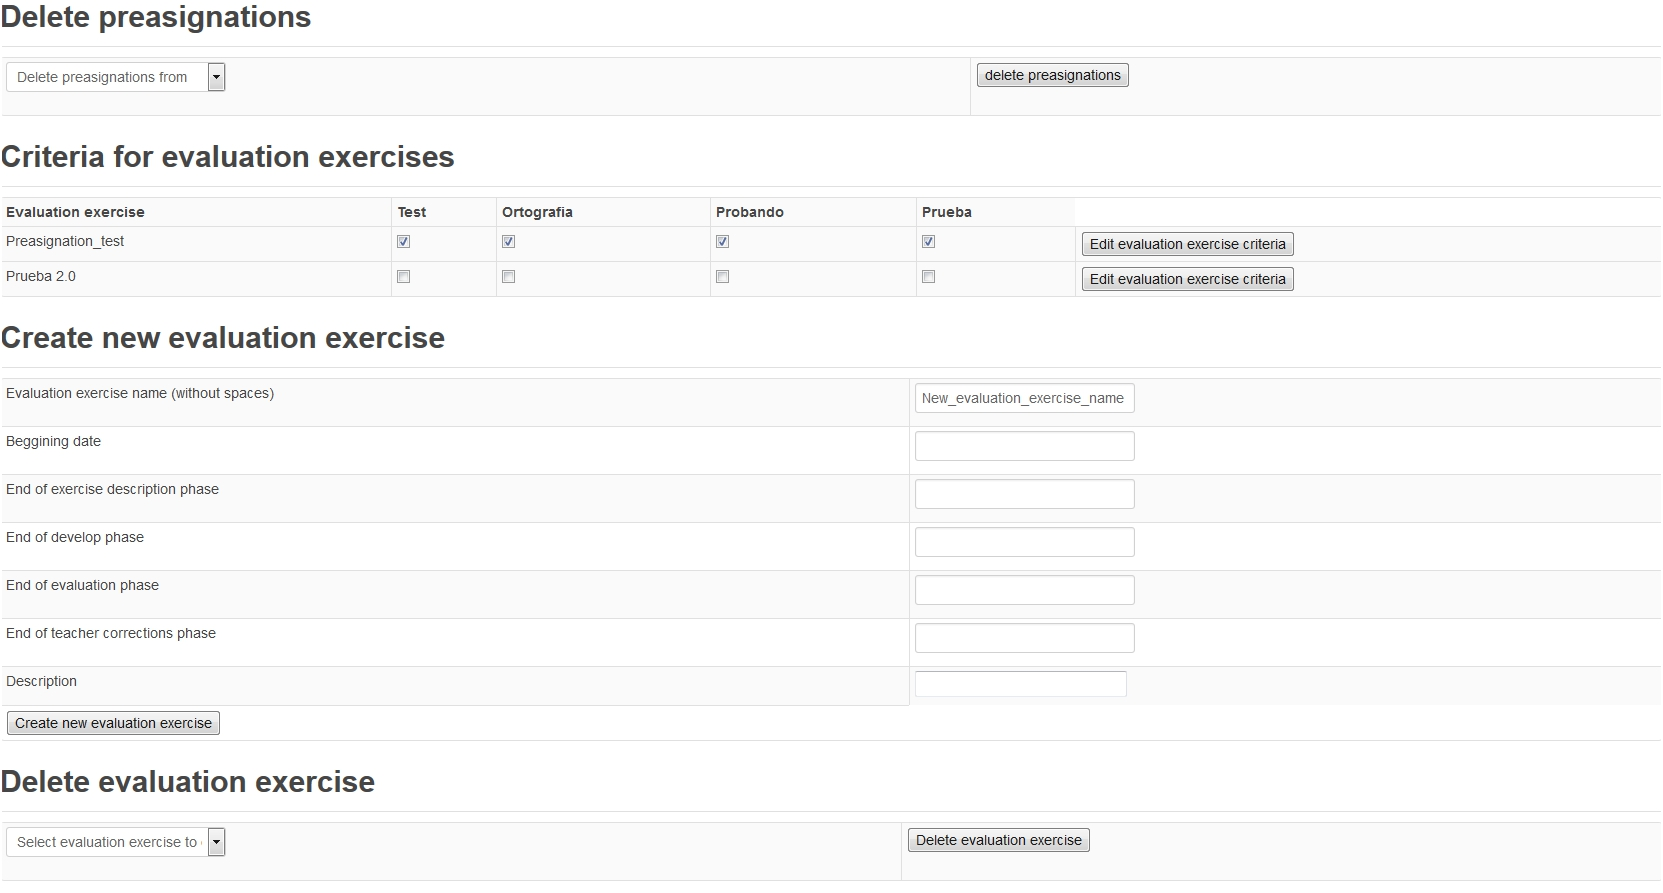
\includegraphics[width=0.9\textwidth]{sc_ee2.jpg}
	\caption{Pantalla de configuración de ejercicios de evaluación.}
\end{figure}
\clearpage

A continuación veremos la interfaz de ayuda extra, accesible desde el botón "Help" al final del listado de parámetros,  en esta nueva interfaz se mostrara información al usuario en caso de que necesite recordar el uso de alguna característica del sistema.\\

\begin{figure}[h!]
	\centering
	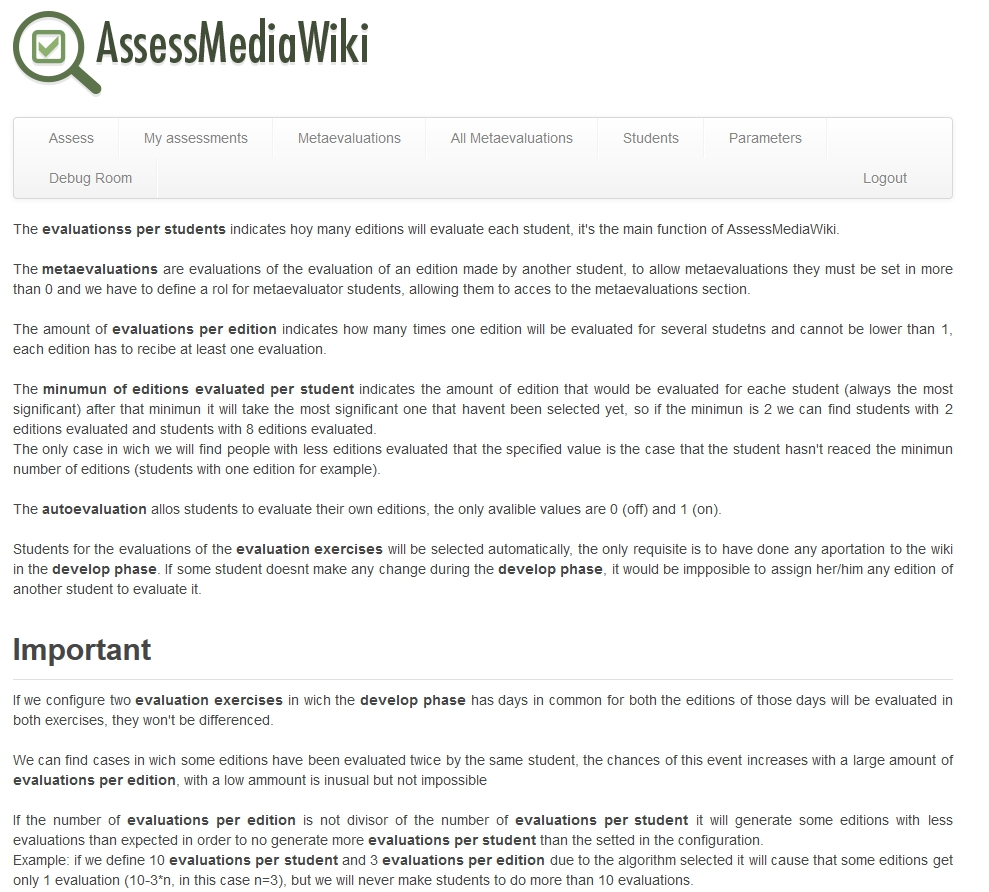
\includegraphics[width=0.9\textwidth]{sc_extra_help.jpg}
	\caption{Pantalla de ayuda extra.}
\end{figure}
\clearpage